The corrosion triggered by carbonation differs substantially from other aggressive mechanisms due to its global chemical nature, governed by the progressive reduction of the cementitious matrix alkalinity. While agents such as chloride ions pierce the passive layer locally (\textit{pitting}), carbonation advances as an acid front that lowers the concrete pH to levels below 9, promoting generalized depassivation of the entire affected reinforcement surface. This large-scale loss of protection results in uniform corrosion, characterized by the voluminous formation of expansive oxides along the bar, which inevitably generates tensile stresses in the concrete, culminating in intense cracking and cover spalling even before critical cross-sectional loss of the steel occurs.

\begin{figure}[htpb!]
    \centering
    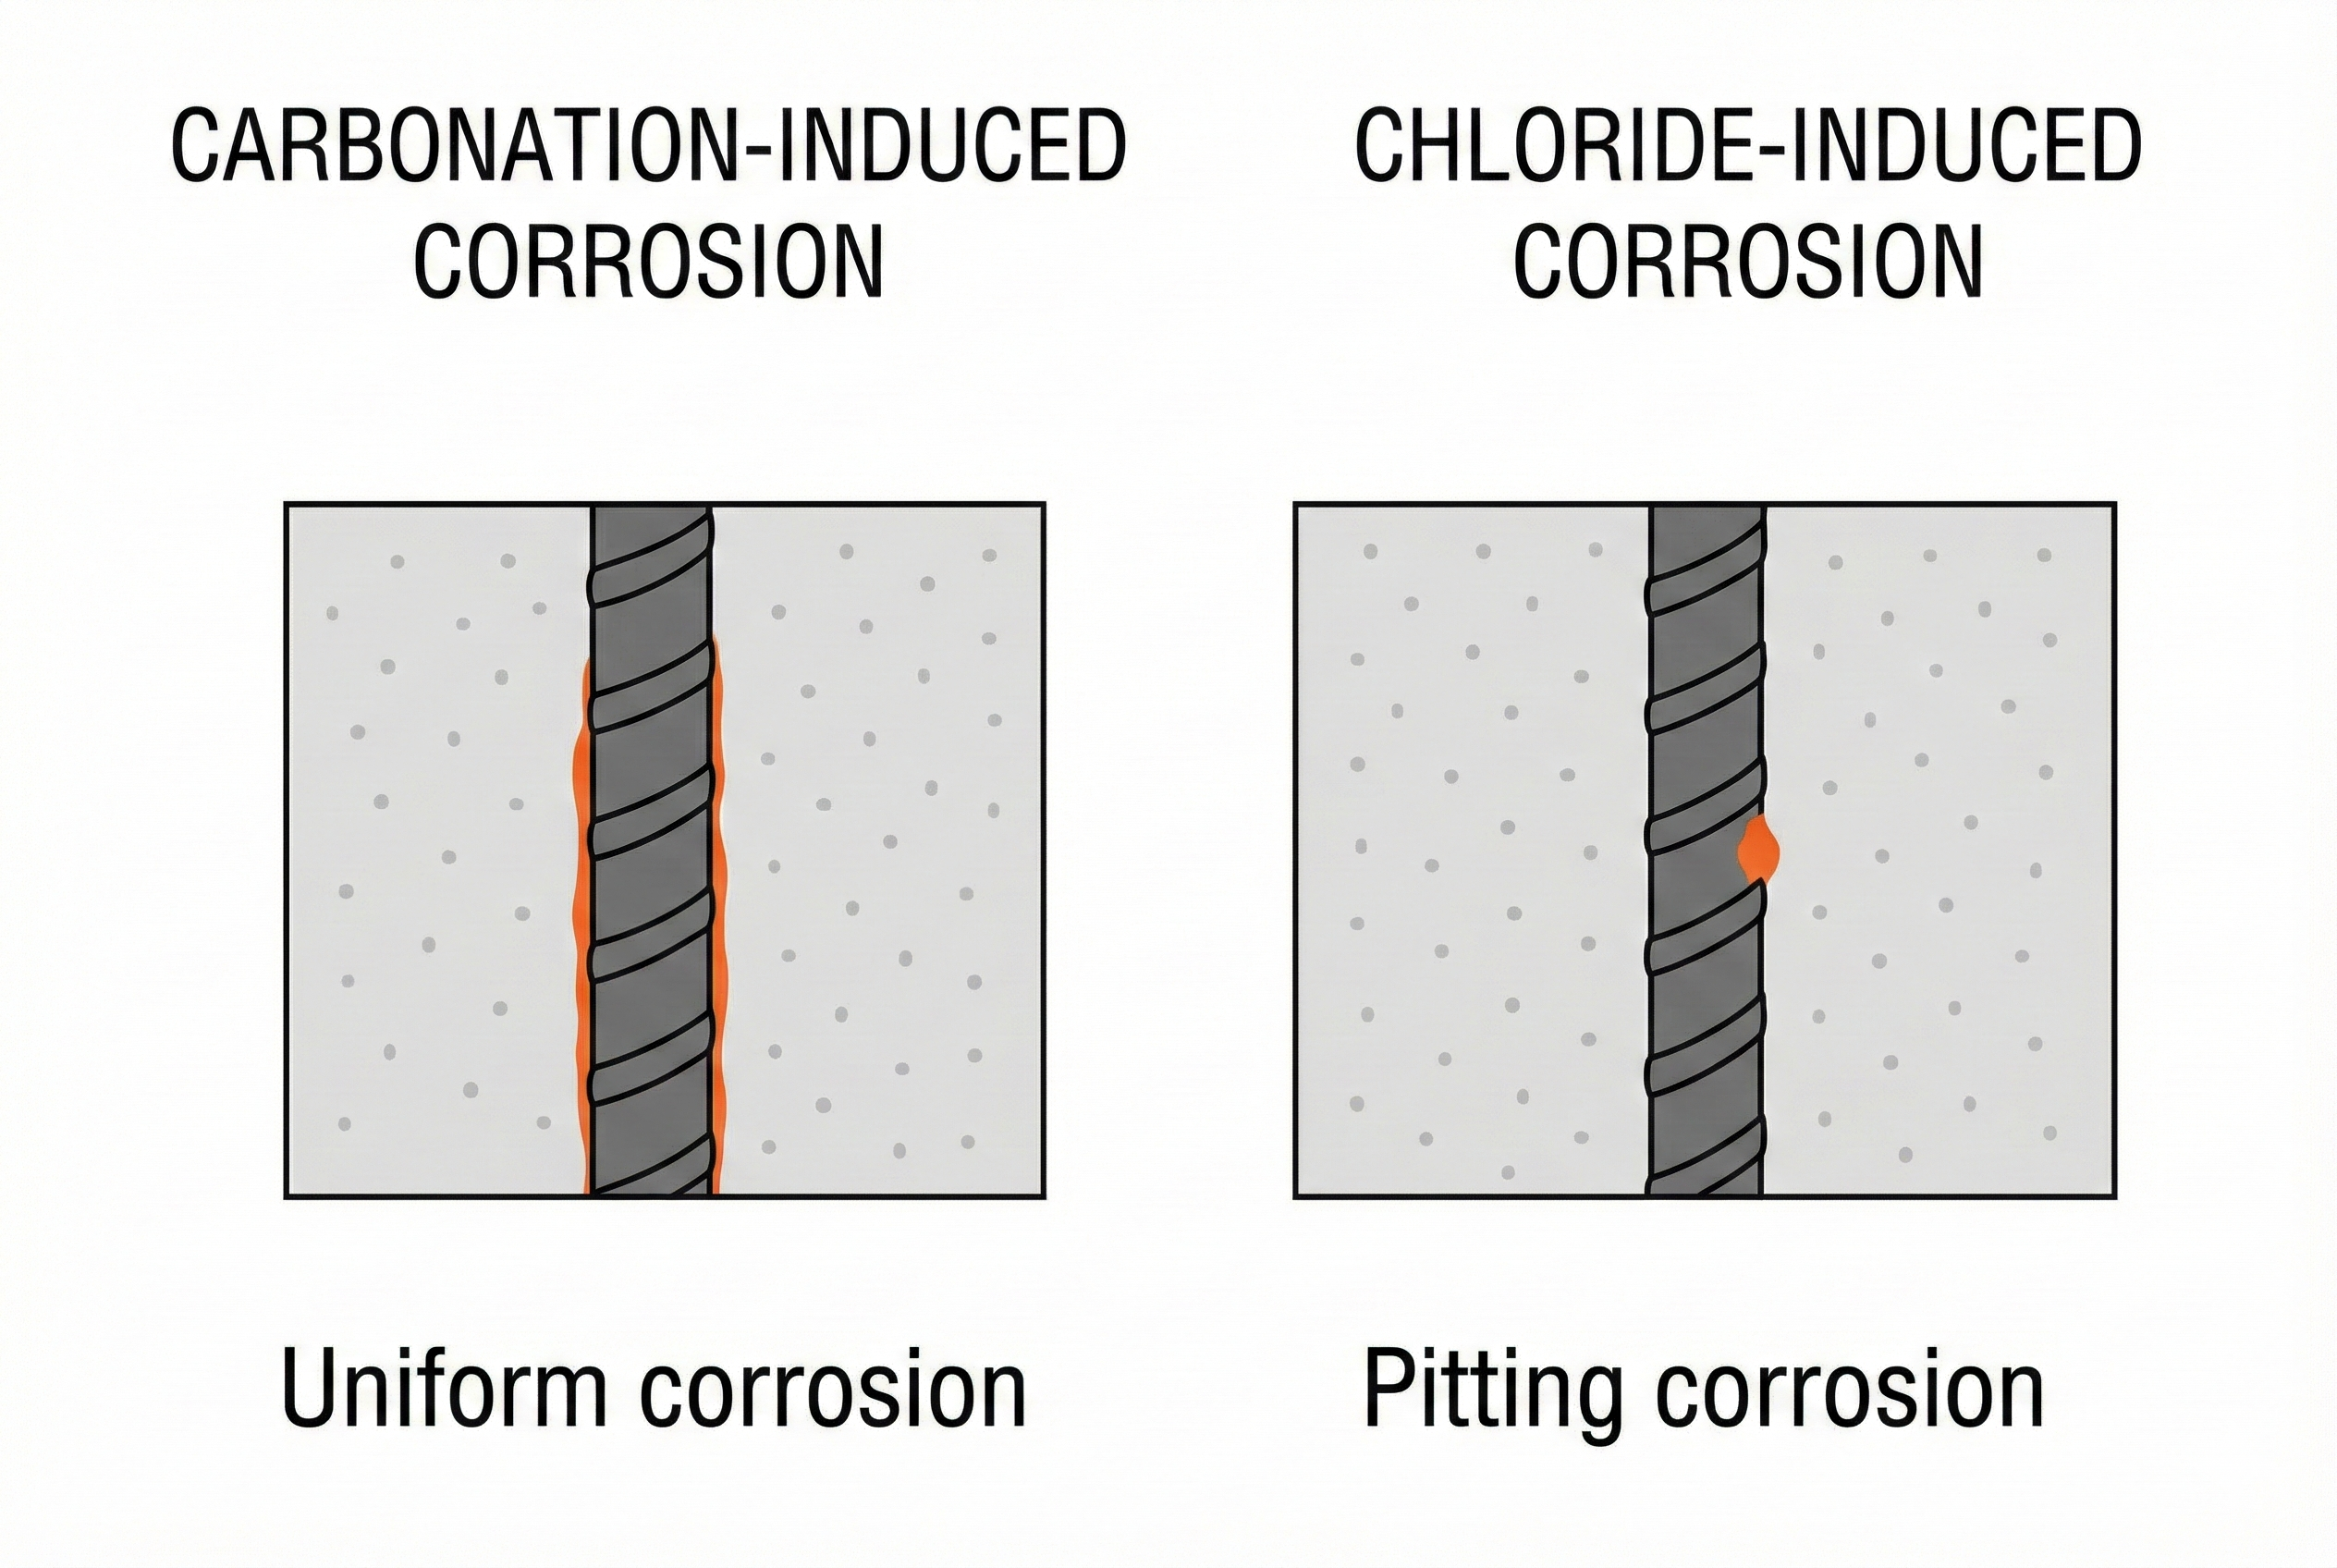
\includegraphics[width=0.5\linewidth]{z_corrosion_en.png}
    \caption{Corrosion differences.}
    \label{fig:z_corrosion_en}
\end{figure}

\subsection{Carbonation-induced corrosion phenomena}
Corrosion of steel reinforcement induced by carbonation represents one of the primary degradation mechanisms in reinforced concrete structures. The process initiates with the diffusion of atmospheric carbon dioxide (CO$_2$) through the concrete pore network. The CO$_2$ subsequently reacts with pore moisture and cement hydration products, predominantly calcium hydroxide (Ca(OH)$_2$), leading to the formation of calcium carbonate (CaCO$_3$).

This chemical reaction induces a substantial reduction in the concrete pore solution pH. Under normal conditions, concrete maintains a highly alkaline environment (pH range: 12.6--13.5), which sustains a stable passive oxide layer on the steel reinforcement surface, providing effective corrosion protection. However, the progressive advancement of the carbonation front reduces the pH to values below 9. This acidification of the concrete matrix initiates the depassivation of the reinforcement, rendering the steel susceptible to generalized corrosion in the presence of sufficient oxygen and moisture.

The speed and depth of carbonation are influenced by various environmental and material factors, such as: CO$_2$ concentration (higher levels accelerate the reaction); Relative Humidity (RH) (carbonation is most intense in intermediate ranges, typically 50\%--70\%); Concrete Quality (water/cement ratio, cement type, and porosity determine CO$_2$ ingress ease); and Cover thickness (acting as a physical barrier).

\subsection{Dataset}

This study employs a comprehensive dataset of carbonation progression in concrete structures, comprising 20,000 samples obtained from \citet{couto_machine_2025}. The dataset incorporates both numerical and categorical variables characterizing environmental conditions, material properties, and temporal factors influencing carbonation depth.

The dataset incorporates seven variables: two categorical and five numerical. The numerical input features encompass atmospheric CO$_2$ concentration (\%), 28-day concrete compressive strength $f_c$ (MPa), environmental relative humidity RH (\%), and exposure duration $t$ (years), while the target variable is the carbonation depth $y$ (mm).

Categorical variables include cement type and exposure conditions. The cement classification adheres to the Brazilian standard ABNT NBR 16697, where the acronym 'CP' denotes Portland Cement, followed by suffixes indicating the predominant supplementary cementitious material: 'E' for blast furnace slag, 'Z' for pozzolan, 'F' for carbonaceous filler, and 'ARI' for High Early Strength. Based on this standardization, the study analyzed six distinct types with varying clinker and supplementary material contents: CP V-ARI (>90\% clinker); CP II-E (70--80\% clinker, 15--25\% slag); CP II-F (70--80\% clinker, 10--20\% limestone); CP II-Z (70--80\% clinker, 15--25\% pozzolan); CP III (25--35\% clinker, 60--70\% slag); and CP IV (55--65\% clinker, 25--40\% pozzolan). Furthermore, environmental exposure conditions are classified as Protected Indoor (PIA), Protected Outdoor (PEA), or Unprotected Outdoor (UEA).

Table~\ref{tab:statistics} presents the basic descriptive statistics for the numerical variables. Figure~\ref{fig:histograms} complements this analysis by showing the distribution of each variable through individual KDE (Kernel Density Estimation), offering visual assessment of data spread and central tendencies. Carbonation depth in millimeters serves as the target variable for subsequent predictive modeling.

\begin{table}[htpb!]
    \centering
    \small
    \caption{Descriptive statistics of numerical variables in the carbonation dataset ($n = 20,000$).}
    \label{tab:statistics}
     \begin{tabular}{lrrrr}
    \toprule
     & \textbf{mean} & \textbf{std} & \textbf{min} & \textbf{max} \\
    \midrule
   \textbf{ CO2 (\%)} & 0.16 & 0.08 & 0.03 & 0.30 \\
   \textbf{ $f_c$ (MPa)} & 34.90 & 8.66 & 20.00 & 50.00 \\
    \textbf{RH (\%)} & 59.94 & 17.31 & 30.00 & 90.00 \\
    \textbf{Type of cement} & 2.51 & 1.71 & 0.00 & 5.00 \\
    \textbf{Exposure conditions} & 0.99 & 0.82 & 0.00 & 2.00 \\
    \textbf{$t$ (years)} & 49.93 & 29.32 & 0.00 & 100.00 \\
    \textbf{carb. depth (mm)} & 16.59 & 12.84 & 0.00 & 119.71 \\
    \bottomrule
    \end{tabular}
\end{table}

\begin{figure}[htpb!]
    \centering
    \begin{subfigure}[b]{0.35\textwidth}
        \centering
        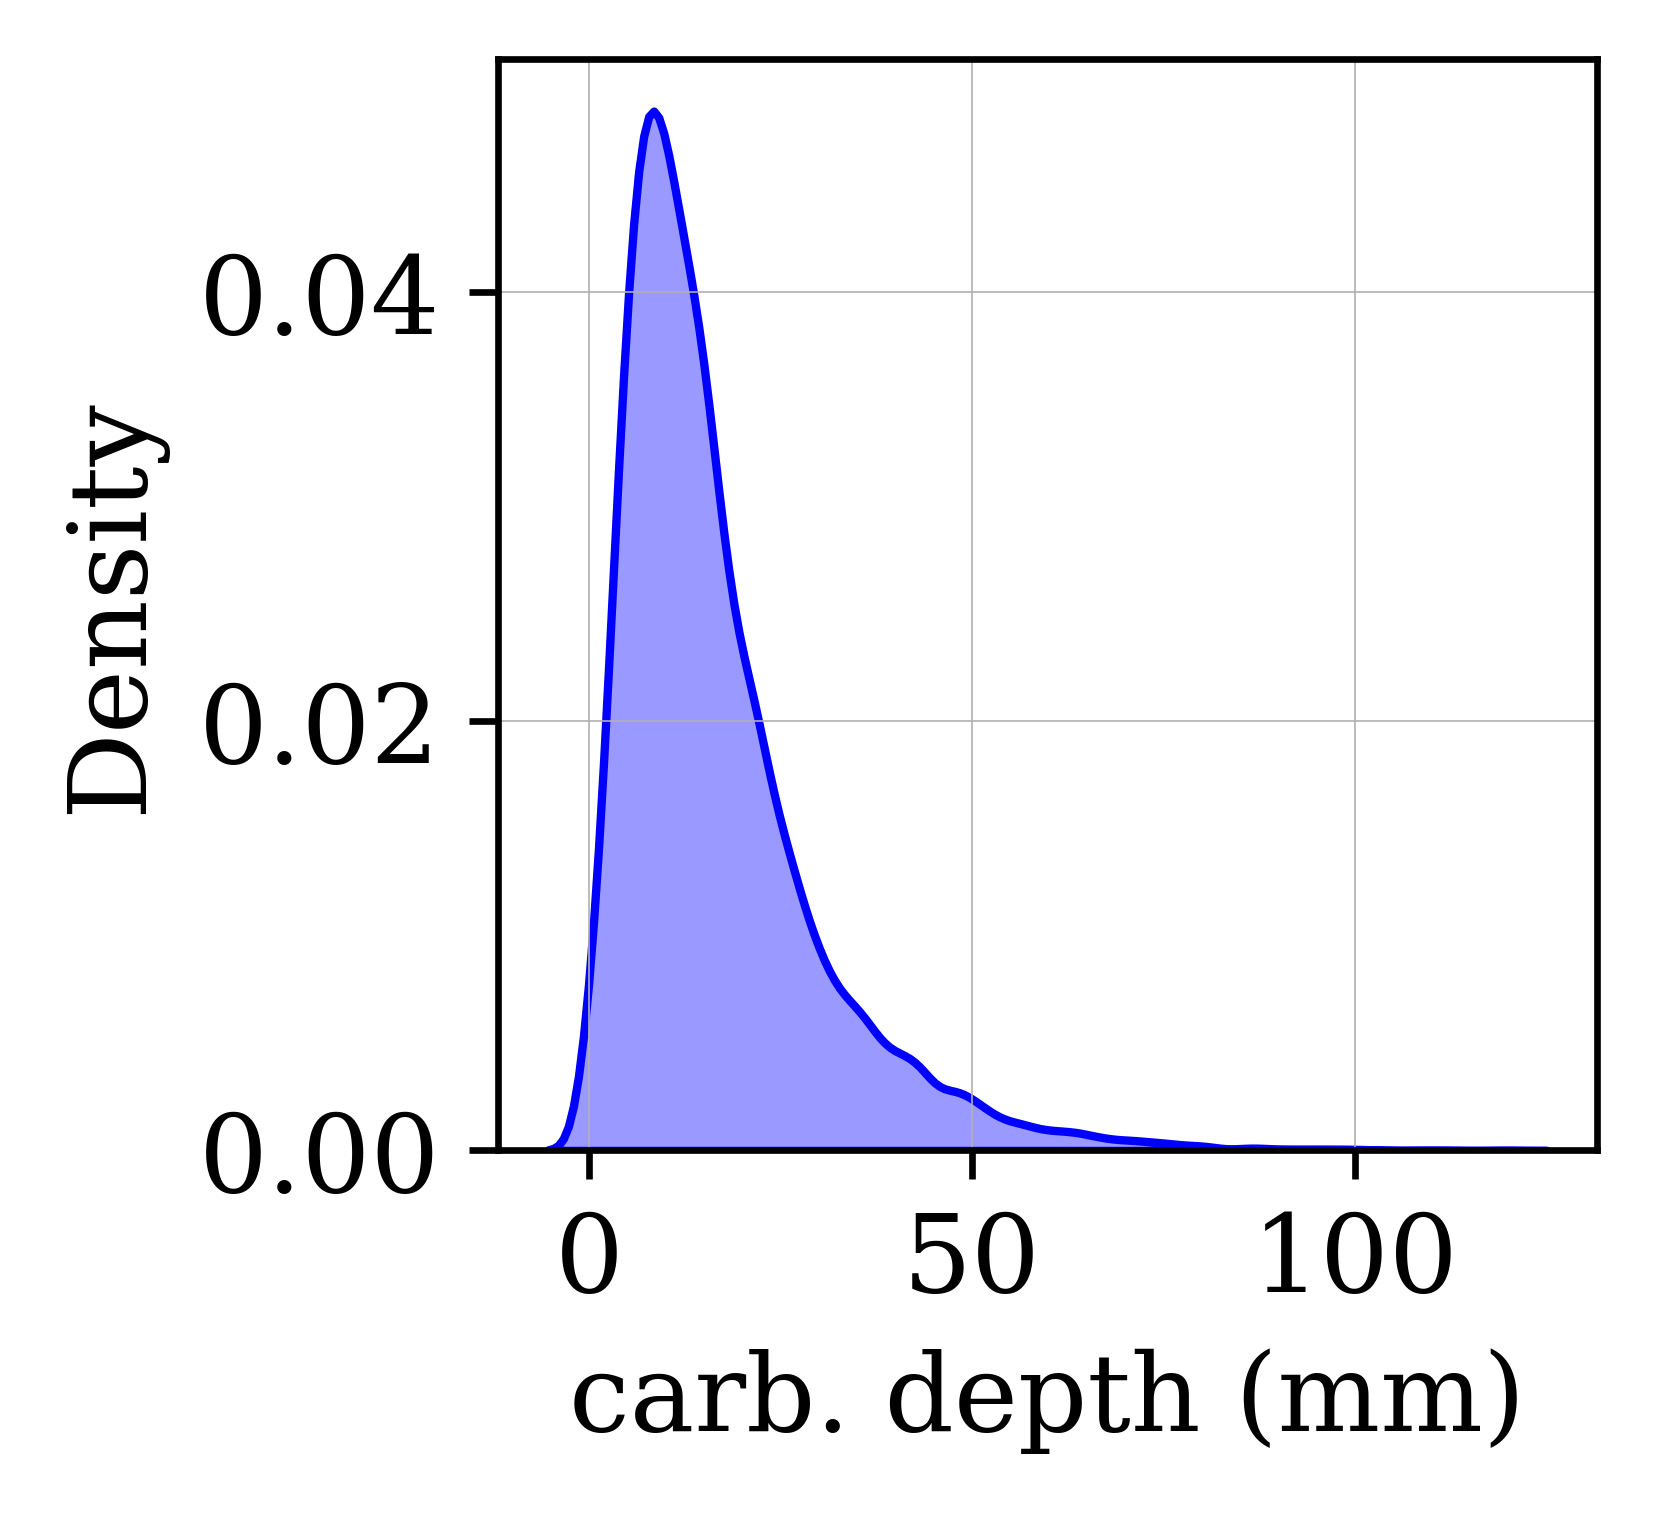
\includegraphics[width=1\linewidth]{z_kde_carbonation_depth.png}
        \caption{CO$_2$ concentration}
        \label{fig:hist_co2}
    \end{subfigure}
    \hfill
    \begin{subfigure}[b]{0.35\textwidth}
        \centering
        
\includegraphics[width=1\linewidth]{z_kde_compressive_strength.png}
        \caption{Concrete strength $f_c$}
        \label{fig:hist_fc}
    \end{subfigure}

    \vspace{0.3cm}

    \begin{subfigure}[b]{0.35\textwidth}
        \centering
        
\includegraphics[width=1\linewidth]{z_kde_relative_humidity.png}
        \caption{Relative humidity RH}
        \label{fig:hist_rh}
    \end{subfigure}
    \hfill
    \begin{subfigure}[b]{0.35\textwidth}
        \centering
        
\includegraphics[width=1\linewidth]{z_kde_time.png}
        \caption{Exposure time $t$}
        \label{fig:hist_time}
   \end{subfigure}

    \vspace{0.3cm}

    \begin{subfigure}[b]{0.35\textwidth}
        \centering
        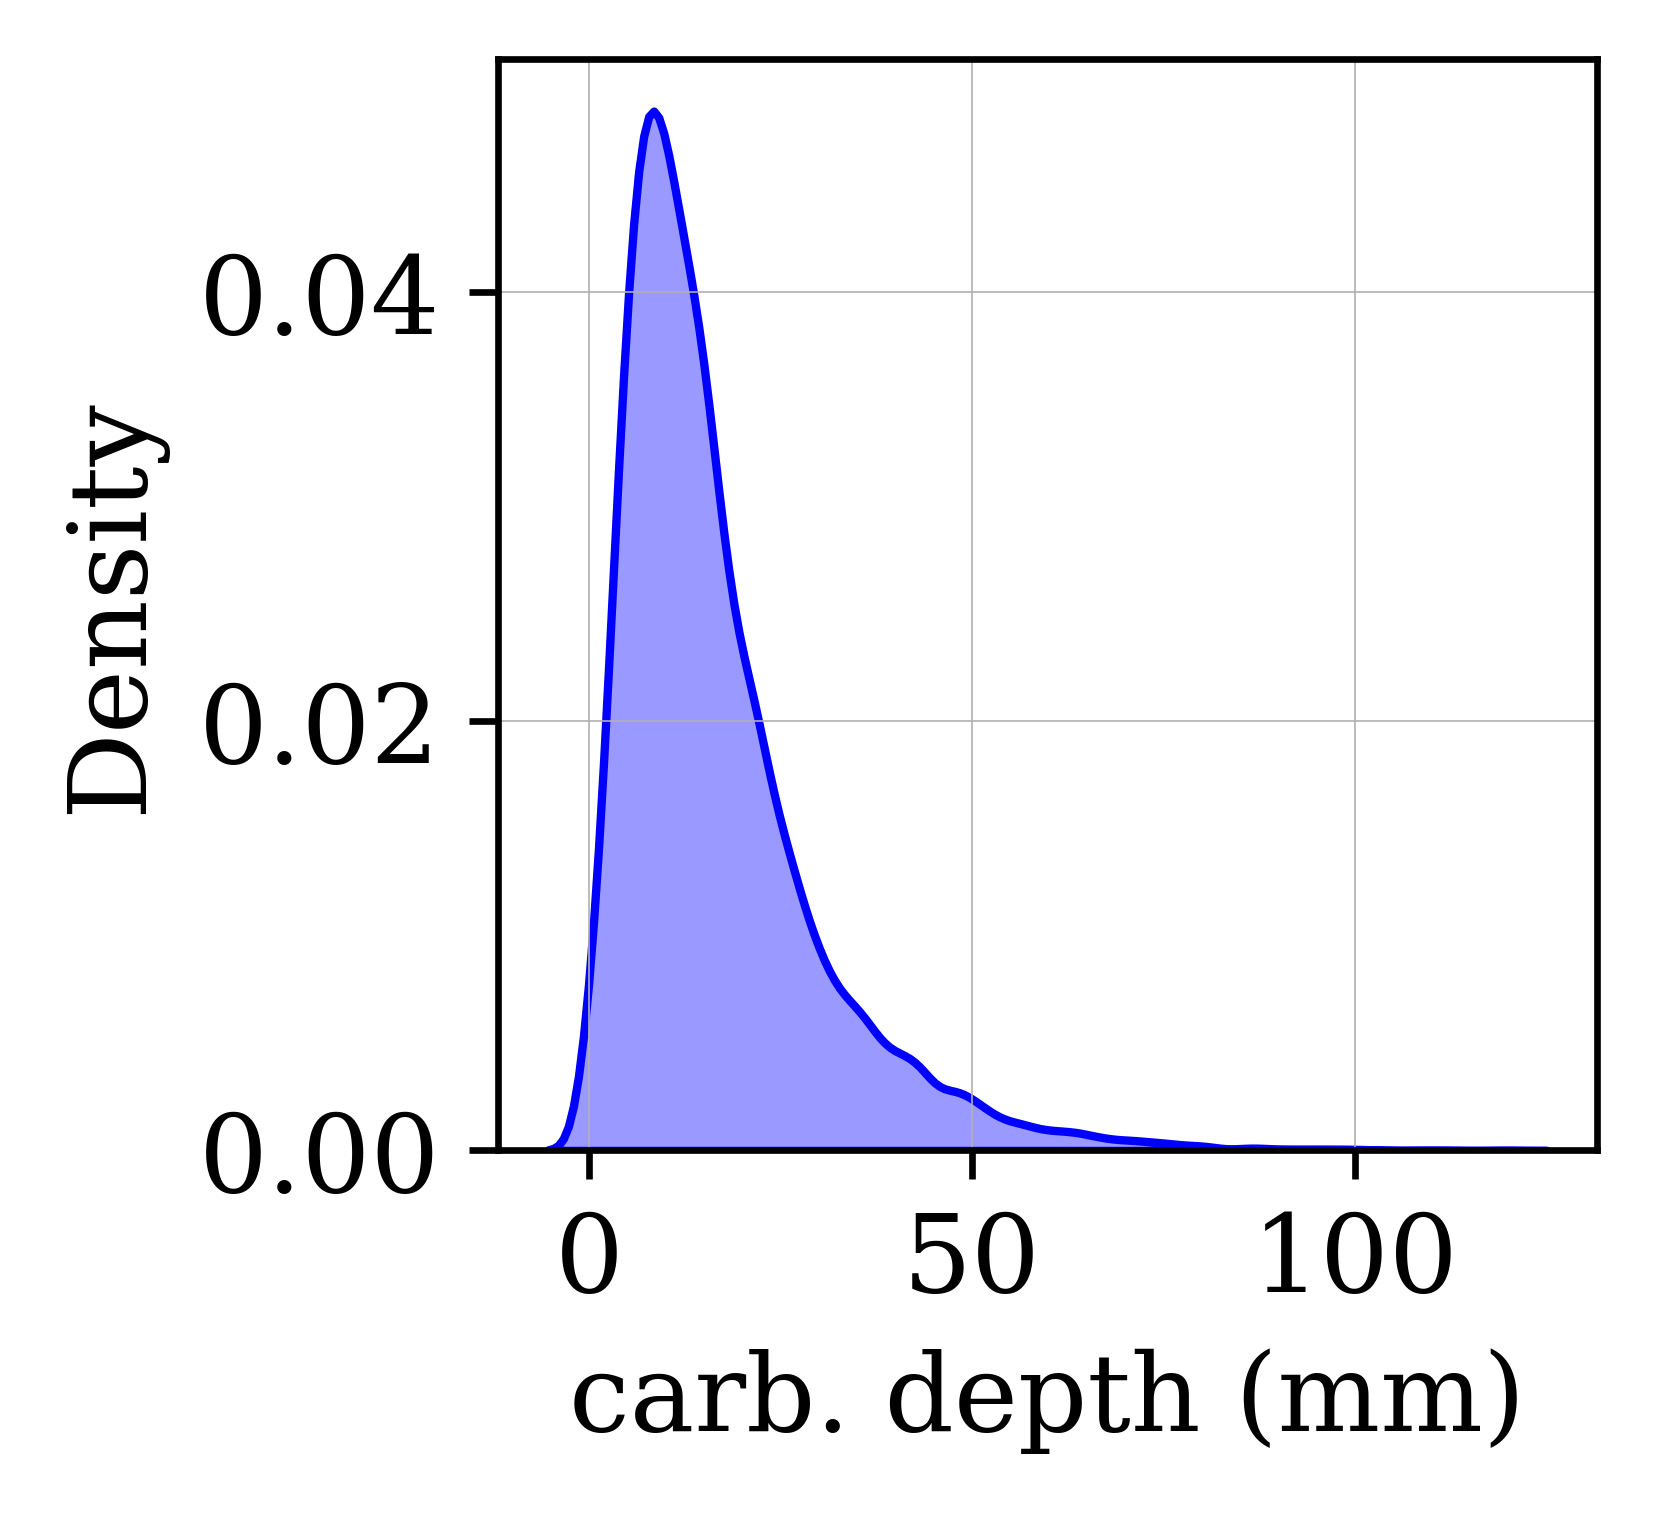
\includegraphics[width=1\linewidth]{z_kde_carbonation_depth.png}
        \caption{Carbonation depth $y$}
        \label{fig:hist_depth}
    \end{subfigure}

    \caption{Kernel Density Estimation (KDE) of numerical variables in the carbonation dataset.}
    \label{fig:histograms}
\end{figure}

The KDE plots reveal the statistical profile of the dataset. The concrete compressive strength ($f_c$) exhibits a multimodal distribution concentrated around commercial classes (20, 30 and 40 MPa). The environmental variables cover a representative range of exposure conditions, while the time variable ($t$) indicates that the dataset includes both young concrete and mature structures, providing a solid temporal basis for regression.

\subsection{Machine Learning approach}

\subsubsection{Training and test}
This study employs supervised machine learning, where algorithms learn a mapping function $f: X \to Y$ from labeled data to minimize prediction error on unseen samples. Among the regression models applied, the Multi-Layer Perceptron (MLP) stands out for its ability to approximate complex non-linear functions. Structurally, an MLP consists of input, hidden, and output layers composed of neurons. Each neuron computes a weighted sum of inputs plus a bias, which is then passed through a non-linear activation function. The network "learns" by iteratively adjusting these weights and biases using the backpropagation algorithm and an optimizer to minimize a specific loss function.

Based on this theoretical framework, the specific model in this work was implemented by feeding the input features directly into the network. The topology was configured with two hidden layers containing 100 and 50 neurons, respectively. The Rectified Linear Unit (ReLU) was employed as the non-linear activation function, while the Adaptive Moment Estimation (Adam) algorithm was selected as the solver for weight optimization.

Seven machine learning models were trained to predict carbonation depth in concrete structures. To ensure statistical robustness and mitigate overfitting, a 10-fold cross-validation strategy was employed. In each iteration, the dataset was randomly split into training (80\%) and testing (20\%) sets. Table~\ref{tab:model_performance} presents the mean $R^2$ scores evaluated on these independent test sets. Figure~\ref{fig:model_comparison} illustrates the comparison between predicted and observed values, with figure (a) showing the worst-performing model and figure (b) displaying the best-performing model.

\begin{table}[H]
    \centering
    \small
    \caption{Performance metrics ($R^2$) of machine learning models on the independent test set (20\% kfold). Values presented as Mean.}
    \label{tab:model_performance}
    \begin{tabular}{lcc}
        \toprule
        \textbf{Model} & \textbf{$R^2$ Train} & \textbf{$R^2$ Test} \\
        \midrule
        Linear Regression & 0.54 & 0.54 \\
        Ridge Regressor & 0.54 & 0.54 \\
        Lasso Regressor & 0.53 & 0.53 \\
        Decision Tree & 1.00 & 0.92 \\
        Random Forest & 0.99 & 0.96 \\
        Gradient Boosting & 0.95 & 0.94 \\
        Hist Gradient Boosting & 0.99 & 0.99 \\
        \textbf{Neural Network MLP} & \textbf{0.99} & \textbf{0.99} \\
        \bottomrule
        \multicolumn{3}{l}{\footnotesize \textit{Note: Standard deviation was omitted due to negligible values (magnitude $\le 1\%$) across all iterations.}} \\
    \end{tabular}

    \vspace{0.2cm}
\end{table}

\begin{figure}[htpb!]
    \centering
    \begin{subfigure}[b]{0.40\textwidth}
        \centering
        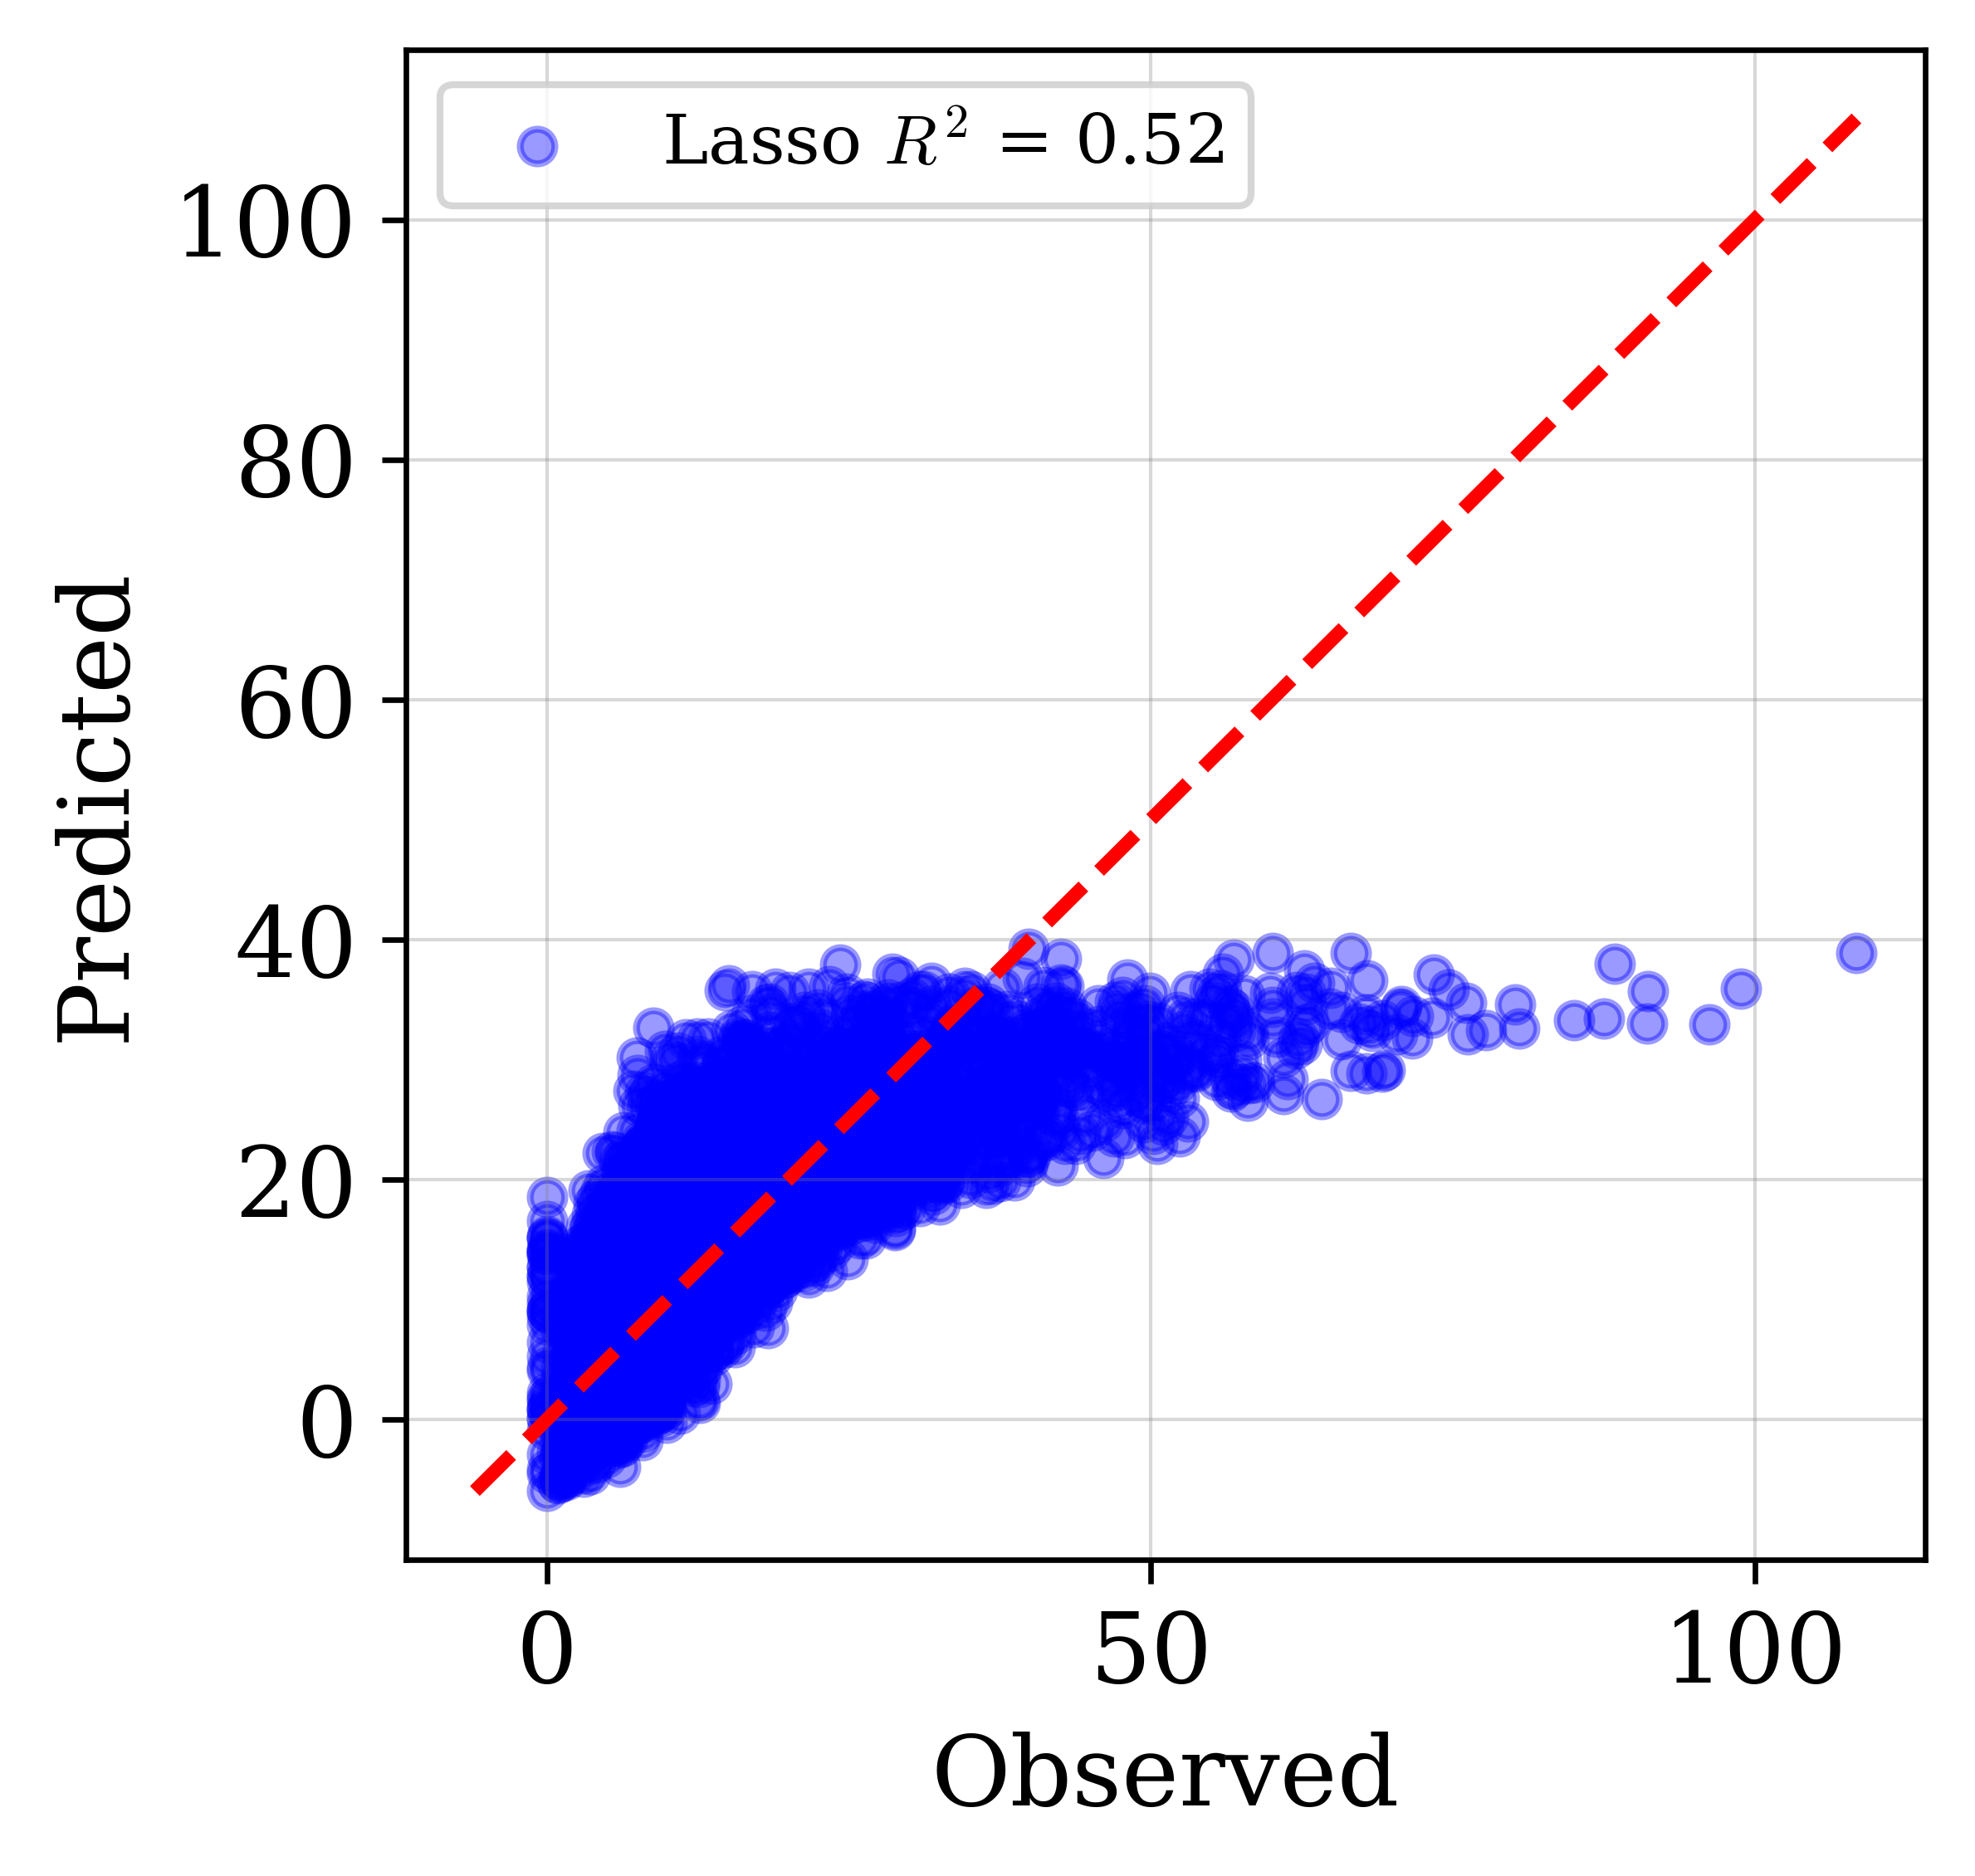
\includegraphics[width=\linewidth]{z_scatter_worst_model_en.png}
        \caption{Worst model: Lasso Regressor ($R^2 = 0.52$)}
        \label{fig:worst_model}
    \end{subfigure}
    \hfill
    \begin{subfigure}[b]{0.375\textwidth}
        \centering
        
\includegraphics[width=\linewidth]{z_scatter_best_model_en.png}
        \caption{Best model: Neural Network MLP ($R^2 = 0.99$)}
        \label{fig:best_model}
    \end{subfigure}
    \caption{Comparison between predicted and observed carbonation depth values for (a) the worst-performing and (b) best-performing models. The dashed line represents perfect prediction ($y=\hat{y}$).}
    \label{fig:model_comparison}
\end{figure}

The Figure \ref{fig:model_comparison} comparison between predicted and observed carbonation depth values for (a) the worst-performing model (Lasso, $R^2$ = 0.52) and (b) best-performing model (Neural Network MLP, $R^2$ = 0.99). The dashed line represents perfect prediction.

\subsubsection{CO2 profile}
To model the temporal evolution of atmospheric carbon dioxide ($CO_2$) concentration, a fundamental parameter for structural degradation simulations, an approach based on historical and instrumental records was adopted. For the initial historical period (1900 to 1950), the dataset derives from high-resolution paleoclimatic records extracted from Antarctic ice cores (Law Dome), which provide critical data covering the pre-industrial period to the 20th century and are managed by the NOAA National Centers for Environmental Information (NOAA/NCEI) \cite{noaa_law_dome}. From 1950 onwards, the model is anchored in continuous direct atmospheric measurements provided by the NOAA Global Monitoring Laboratory (GML) at the Mauna Loa observatory in Hawaii \cite{noaa_gml}, alongside records from the World Data Centre for Greenhouse Gases (WDCGG) \cite{wmo_wdcgg}.

For use in this research, a piecewise analytical regression was created to simulate this $CO_2$ accumulation profile, yielding a coefficient of determination ($R^2$) of 0.99. The mathematical framework divides the time series into three continuous regimes of anthropogenic growth, illustrated in Figure \ref{fig:evolution_co2}. These include a slow linear growth between 1900 and 1950, an accelerated linear growth between 1950 and 2000, and a quadratic growth post-2000, capturing the contemporary intensification of global emissions.

To illustrate the practical application of the described models, parametric simulations were conducted projecting the carbonation advancement for the extended period from 1900 to 2150. The subsequent graphs present the temporal evolution of the carbonation front, highlighting the direct influence of the concrete compressive strength class ($f_{ck}$) (Figure \ref{fig:evolution_fck}) and the environmental relative humidity (Figure \ref{fig:evolution_h}) on the degradation rate. For service life assessment purposes, a reference line was set at 30 mm, corresponding to a typical normative concrete cover \cite{nbr6118}, indicating the theoretical threshold for reinforcement depassivation.

\begin{figure}
    \centering
    
\includegraphics[width=0.5\linewidth]{z_graph_1900_co2.png}
    \caption{Evolution of Carbonation by $CO_2$}
    \label{fig:evolution_co2}
\end{figure}

Figure \ref{fig:evolution_co2} piecewise regression curve of atmospheric carbon dioxide ($CO_2$) concentration simulated from 1900 to 2150. The graph illustrates the model's transitions between the slow linear historical regime (pre-1950), the accelerated linear regime (1950–2000), and the contemporary quadratic non-linear behavior (post-2000) projecting future accumulations.

\begin{figure}
    \centering
    
\includegraphics[width=0.5\linewidth]{z_graph_1900_fck.png}
    \caption{Evolution of Carbonation by $fck$}
    \label{fig:evolution_fck}
\end{figure}

Figure \ref{fig:evolution_fck} temporal evolution of carbonation depth for different compressive strength classes ($f_{ck}$), considering a constant relative humidity of 65\% (critical scenario) and a normative concrete cover of 30 mm, simulated for the period from 1900 to 2150.

\begin{figure}
    \centering
    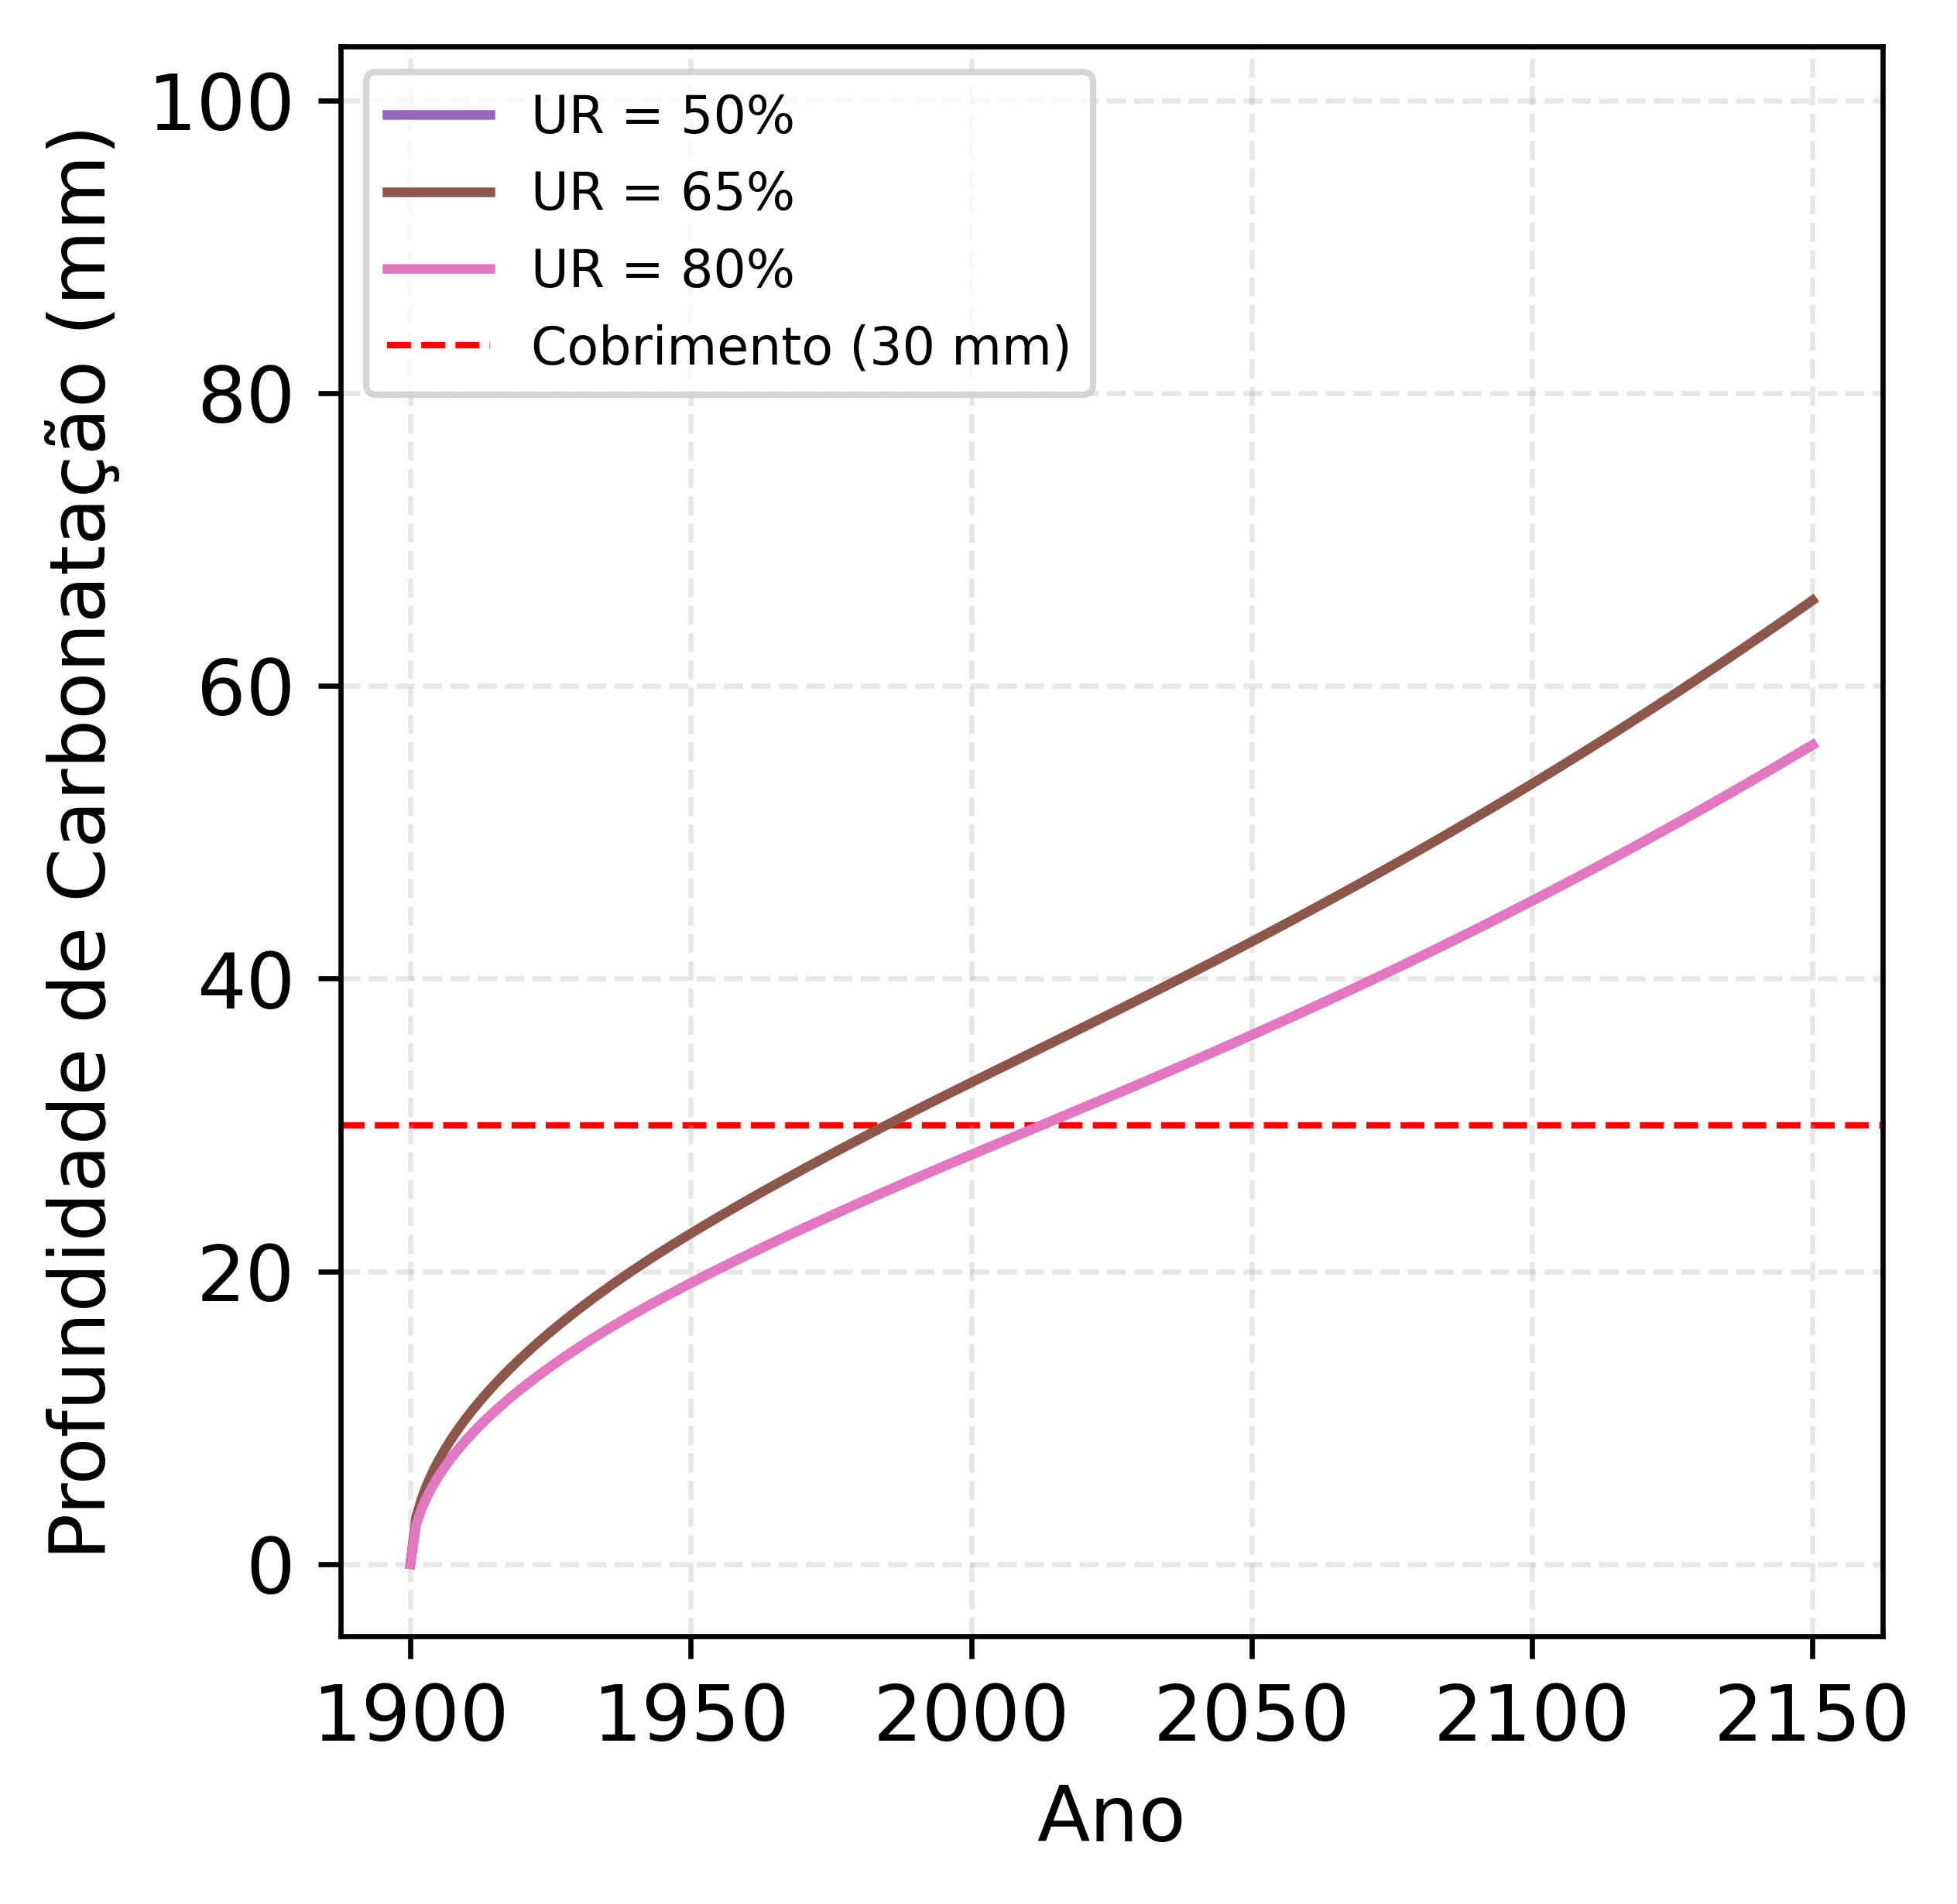
\includegraphics[width=0.5\linewidth]{z_graph_1900_h.png}
    \caption{Evolution of Carbonation by humidity}
    \label{fig:evolution_h}
\end{figure}

Figure \ref{fig:evolution_h} influence of relative humidity on the advancement of the carbonation front over time for concrete with an $f_{ck}$ of 30 MPa. The graph highlights the acceleration of degradation in environments with intermediate humidity (65\%) compared to drier (50\%) or more humid (80\%) environments, simulated for the period from 1900 to 2150.

\subsubsection{Carbonation profile}

Carbonation depth profiles were analyzed to determine the carbonation coefficient ($k$), a key parameter characterizing the rate of carbonation progression. The coefficient $k$ is obtained by rearranging the carbonation depth law (Equation as $k = y / \sqrt{t}$, where $y$ represents carbonation depth (mm) and $t$ denotes exposure time (years).
Figure \ref{fig:z_carbonation_profile} presents the average carbonation coefficient along with four representative carbonation depth profiles. The figure illustrates profiles for indoor exposure conditions (AIP), which exhibited the highest carbonation rates across all strength classes. 

\begin{figure}[htpb!]
        \centering
        
\includegraphics[width= 0.60\textwidth]{z_carbonation_profile.png}
        \caption{Indoor exposure (AIP) profiles. Carbonation coefficients: k20 = 5.8, k30 = 3.8, k40 = 2.3, k50 = 1.7 mm/sqrt(year)}
        \label{fig:z_carbonation_profile}
    \end{figure}

    
\subsection{Machine Learning}

Machine Learning (ML) is a subfield of Artificial Intelligence focused on the development of algorithms capable of learning patterns and making inferences from data without being explicitly programmed for specific rules. Unlike the traditional deterministic approach, where an expert defines the physical equations governing the phenomenon, ML models induce mathematical relationships directly from empirical observations.

This paradigm relies on generalization capability: the algorithm analyzes a training dataset to construct a model capable of making accurate predictions on new, unseen data. ML techniques are broadly categorized into supervised, unsupervised, and reinforcement learning. In the context of predicting the service life of structures, supervised learning is predominant. Here, the model is trained with known input-output pairs, enabling the mapping of complex, non-linear interactions that often elude conventional analytical formulations.

\subsection{Neural Networks}

Artificial Neural Networks (ANNs) are computational models inspired by the biological neural networks of the human brain. As a fundamental subset of machine learning and deep learning, ANNs are designed to recognize complex patterns, map non-linear relationships, and process large volumes of data. The architecture of a standard neural network is structured into three main parts: an input layer, one or more hidden layers, and an output layer. These layers are composed of interconnected nodes, known as artificial neurons, which process information by applying synaptic weights and activation functions. During the training phase, the network employs optimization algorithms, such as backpropagation, to iteratively adjust these mathematical weights in order to minimize the loss function (error). This continuous adjustment process grants the model the ability to autonomously learn and generalize solutions from the provided data.

\subsection{Theoretical Background: Histogram-based Gradient Boosting Regressor (HGBR)}

The \textit{Histogram-based Gradient Boosting Regressor} (HGBR) is an advanced machine learning technique belonging to the \textit{Gradient Boosting Decision Trees} (GBDT) family. This approach is grounded in the principle of ensemble learning, where multiple simple predictive models—termed "weak learners"—are combined sequentially to form a robust and high-precision predictor.

\subsubsection{Boosting Mechanism}

The core operation of the algorithm is based on the additive construction of decision trees. Unlike models such as \textit{Random Forest}, which build independent trees in parallel, HGBR constructs trees sequentially. Each new tree is trained specifically to correct the residual errors (the difference between the actual and predicted values) made by the ensemble of previous trees.

Mathematically, the final prediction $\hat{y}_i$ for a given input $x_i$ is the sum of the predictions of $K$ trees:

\begin{equation}
    \hat{y}_i = \sum_{k=1}^{K} f_k(x_i), \quad f_k \in \mathcal{F}
\end{equation}

Where $\mathcal{F}$ represents the function space of all possible regression trees. The optimization process seeks to minimize an objective function at each iteration $t$, composed of a differentiable loss function $l$ (such as Mean Squared Error) and a regularization term $\Omega$:

\begin{equation}
    \mathcal{Obj}^{(t)} = \sum_{i=1}^{n} l(y_i, \hat{y}_i^{(t-1)} + f_t(x_i)) + \Omega(f_t)
\end{equation}

\subsubsection{Histogram Strategy}

The main innovation of HGBR lies in its computational efficiency. Traditional \textit{Gradient Boosting} algorithms require sorting all values of each continuous feature to find the ideal split point at every tree node, resulting in a high computational cost of $\mathcal{O}(n \log n)$, where $n$ is the number of samples.

HGBR overcomes this limitation through the \textbf{discretization of data into histograms} (hence the name \textit{Histogram-based}). The algorithm groups continuous input variable values into discrete integer bins, typically limited to 256 values (8 bits). 

The process proceeds through a sequence of optimized stages. Initially, via \textbf{Binning (Mapping)}, continuous variables are mapped to discrete integers $b \in \{0, \dots, B-1\}$, where $B$ is the maximum number of bins, drastically reducing the cardinality of the analyzed data. Subsequently, during \textbf{Histogram Construction}, for each tree node, the algorithm constructs a histogram that accumulates the gradients ($g$) and hessians ($h$)—the first and second derivatives of the loss function—for each bin, an operation with linear complexity $\mathcal{O}(n)$. Following this, in the \textbf{Split Finding} phase, instead of iterating over all individual samples, the tree seeks the best split point by iterating only over the histogram bins, reducing the complexity to $\mathcal{O}(B)$, where $B \ll n$. Finally, to further accelerate training, the algorithm utilizes \textbf{Histogram Subtraction}, where the histogram of a child node is calculated by simply subtracting the sibling node's histogram from the parent node's histogram ($Hist_{child} = Hist_{parent} - Hist_{sibling}$), thereby eliminating the need to rescan the data.

\subsubsection{Handling of Missing Values}

An intrinsic feature of this architecture is its native support for missing values. During training, samples with missing data do not need to be imputed. The algorithm automatically learns, for each decision point, whether these samples should be directed to the left or right branch of the tree, based on which direction maximizes the reduction of the loss function (information gain).

This combination of sequential boosting, efficient discretization, and robust data handling makes HGBR capable of modeling complex non-linearities with high training speed and low memory consumption.

\subsection{Performance Evaluation Metrics}

The effectiveness of the proposed regression models was quantified using two complementary statistical metrics: the Coefficient of Determination ($R^2$) and the Adjusted Coefficient of Determination ($R^2_{adj}$). The use of these metrics allows for assessing the model's explanatory capacity weighted by its complexity.

The Coefficient of Determination ($R^2$) indicates the proportion of variance in the dependent variable (carbonation depth) that is predictable from the independent variables. Values range from 0 to 1, where values close to 1 indicate that the model captured most of the patterns present in the data, as shown in Equation \ref{eq:r2}:

\begin{equation}
    R^2 = 1 - \frac{\sum_{i=1}^{n} (y_i - \hat{y}_i)^2}{\sum_{i=1}^{n} (y_i - \bar{y})^2}
    \label{eq:r2}
\end{equation}

Where $y_i$ is the observed value, $\hat{y}_i$ is the predicted value, and $\bar{y}$ is the mean of the observed values.

However, the traditional $R^2$ tends to increase mechanically with the addition of new variables to the model, even if they lack statistical relevance. To mitigate this bias, the Adjusted $R^2$ ($R^2_{adj}$) is used, which incorporates a penalty based on the number of predictors. This metric offers a fairer assessment of the model's generalization and is calculated according to Equation \ref{eq:r2_adj}:

\begin{equation}
    R^2_{adj} = 1 - (1 - R^2) \frac{n - 1}{n - p - 1}
    \label{eq:r2_adj}
\end{equation}

Where $n$ represents the total number of samples and $p$ is the number of independent variables (features) in the model. Thus, an increase in the $R^2_{adj}$ value confirms that the complexity added to the model resulted in a real gain in predictive capacity.

\subsubsection{Relative Entropy or Kullback–Leibler divergence}

Considere uma variável aleatória discreta $X$   com função massa de probabilidade
\[
p(x)=P(X=x), \qquad x \in X.
\]

A entropia relativa ou distância de Kullback--Leibler entre duas
funções de massa de probabilidade $p(x)$ e $q(x)$ é definida por \cite{cover2006elements}
\begin{equation}
D(p\|q)
=
\sum_{x \in \mathcal{X}} p(x)
\log \frac{p(x)}{q(x)}
\label{eq:kl_discreta}
\end{equation}


Na definição acima, utilizamos a convenção de que
$$
0 \log \frac{0}{0} = 0, \ \ \ \ 0 \log \frac{0}{q} = 0 \ \  \text{e} \ \ \ p \log \frac{p}{0} = \infty.
$$
 
 
Assim, se existir algum símbolo $x \in  X $ tal que
$p(x) > 0$ e $q(x)=0$, então
\[
D(p\|q)=\infty.
\]
%%%%%%%%%%%%%%%%%%%%%% 
  Para o caso contínuo, a entropia
relativa ou divergência de Kullback--Leibler entre duas funções densidades de
probabilidade $p(x)$ e $q(x)$ é definida por
\begin{equation}
D(p\|q)
=
\int p(x)\log\frac{p(x)}{q(x)}\,dx.
\label{eq:kl_continua}
\end{equation}

%%%%%%%%%%%%%%%%%%%%%%%%%%%%%%%%%
A entropia relativa é sempre não negativa e é igual a zero se, e somente se,
$p=q$. ela  não é simétrica e não satisfaz a desigualdade triangular. Ainda assim,
é frequentemente útil interpretar a entropia relativa como uma medida de
``distância'' entre distribuições \cite{cover2006elements}.

